
%\documentclass[a4paper,11pt,twoside]{ThesisStyle}
\documentclass[a4paper,11pt,twoside]{article}

\title{First round comments from the Ad-hoc rewiew committee \\
 (Maurik Holtrop, Kevin Giovankl, Zein-Eddine Meziani)}


\date{\today}
\usepackage{amsmath,amssymb}             % AMS Math
% \usepackage[french]{babel}
\usepackage[latin1]{inputenc}
\usepackage[OT1]{fontenc}
\usepackage[left=2.7cm,right=1.7cm,top=1.6cm,bottom=1.6cm,includefoot,includehead,headheight=13.6pt]{geometry}
\usepackage{setspace}
\usepackage{epigraph}
\usepackage{lineno}


%\usepackage{arev}
%\usepackage[bitstream-charter]{mathdesign}
%\usepackage[urw-garamond]{mathdesign}
%\usepackage[sfmath]{kpfonts} %% sfmath option only to make math in sans serif. Probablye only for use when base font is sans serif.
%\renewcommand*\familydefault{\sfdefault} %% Only if the base font of the document is to be sans serif
\usepackage[sc]{mathpazo}
\linespread{1.05}   
\usepackage[T1]{fontenc}



% Table of contents for each chapter

\usepackage[nottoc, notlof, notlot]{tocbibind}
\usepackage{minitoc}
\setcounter{minitocdepth}{2}
\mtcindent=15pt
% Use \minitoc where to put a table of contents

\usepackage{aecompl}

% Glossary / list of abbreviations

\usepackage[intoc]{nomencl}
\renewcommand{\nomname}{List of Abbreviations}

\makenomenclature

% My pdf code

\usepackage{graphicx,type1cm,eso-pic,color}
\usepackage{lscape}

  \usepackage[pagebackref,hyperindex=true]{hyperref}

%\geometry{letterpaper}
%\graphicspath{{.}{images/}}

% nicer backref links
\renewcommand*{\backref}[1]{}
\renewcommand*{\backrefalt}[4]{%
\ifcase #1 %
(Not cited.)%
\or
(Cited on page~#2.)%
\else
(Cited on pages~#2.)%
\fi}
\renewcommand*{\backrefsep}{, }
\renewcommand*{\backreftwosep}{ and~}
\renewcommand*{\backreflastsep}{ and~}

% Links in pdf
\usepackage{color}
\definecolor{linkcol}{rgb}{0,0,0.4} 
\definecolor{citecol}{rgb}{0.5,0,0} 

% Change this to change the informations included in the pdf file

% See hyperref documentation for information on those parameters

\hypersetup
{
bookmarksopen=true,
pdftitle="",
pdfauthor="", pdfsubject="", %subject of the document
%pdftoolbar=false, % toolbar hidden
pdfmenubar=true, %menubar shown
pdfhighlight=/O, %effect of clicking on a link
colorlinks=true, %couleurs sur les liens hypertextes
pdfpagemode=None, %aucun mode de page
pdfpagelayout=SinglePage, %ouverture en simple page
pdffitwindow=true, %pages ouvertes entierement dans toute la fenetre
linkcolor=linkcol, %couleur des liens hypertextes internes
citecolor=citecol, %couleur des liens pour les citations
urlcolor=linkcol %couleur des liens pour les url
}

% definitions.
% -------------------

\setcounter{secnumdepth}{3}
\setcounter{tocdepth}{2}

% Some useful commands and shortcut for maths:  partial derivative and stuff
\newcommand{\xbp}{$x_{Bj}$}
\newcommand{\xb}{$x_{Bj}~$}
\newcommand{\ptp}{$p_\perp^2$}
\newcommand{\pt}{$p_\perp^2~$}
\newcommand{\dptp}{$\Delta \langle p_\perp^2 \rangle$}
\newcommand{\dpt}{$\Delta \langle p_\perp^2 \rangle ~$}

\brokenpenalty10000\relax

\newcommand{\pd}[2]{\frac{\partial #1}{\partial #2}}
\def\abs{\operatorname{abs}}
\def\argmax{\operatornamewithlimits{arg\,max}}
\def\argmin{\operatornamewithlimits{arg\,min}}
\def\diag{\operatorname{Diag}}
\newcommand{\eqRef}[1]{(\ref{#1})}

\usepackage{rotating}                    % Sideways of figures & tables
%\usepackage{bibunits}
%\usepackage[sectionbib]{chapterbib}          % Cross-reference package (Natural BiB)
%\usepackage{natbib}                  % Put References at the end of each chapter
                                         % Do not put 'sectionbib' option here.
                                         % Sectionbib option in 'natbib' will do.
\usepackage{fancyhdr}                    % Fancy Header and Footer

% \usepackage{txfonts}                     % Public Times New Roman text & math font
  
%%% Fancy Header %%%%%%%%%%%%%%%%%%%%%%%%%%%%%%%%%%%%%%%%%%%%%%%%%%%%%%%%%%%%%%%%%%
% Fancy Header Style Options

\pagestyle{fancy}                       % Sets fancy header and footer
\fancyfoot{}                            % Delete current footer settings

%\renewcommand{\chaptermark}[1]{         % Lower Case Chapter marker style
%  \markboth{\chaptername\ \thechapter.\ #1}}{}} %

%\renewcommand{\sectionmark}[1]{         % Lower case Section marker style
%  \markright{\thesection.\ #1}}         %

\fancyhead[LE,RO]{\bfseries\thepage}    % Page number (boldface) in left on even
% pages and right on odd pages
\fancyhead[RE]{\bfseries\nouppercase{\leftmark}}      % Chapter in the right on even pages
\fancyhead[LO]{\bfseries\nouppercase{\rightmark}}     % Section in the left on odd pages

\let\headruleORIG\headrule
\renewcommand{\headrule}{\color{black} \headruleORIG}
\renewcommand{\headrulewidth}{1.0pt}
\usepackage{colortbl}
\arrayrulecolor{black}

\fancypagestyle{plain}{
  \fancyhead{}
  \fancyfoot{}
  \renewcommand{\headrulewidth}{0pt}
}

%\usepackage{algorithm}
%\usepackage[noend]{algorithmic}

%%% Clear Header %%%%%%%%%%%%%%%%%%%%%%%%%%%%%%%%%%%%%%%%%%%%%%%%%%%%%%%%%%%%%%%%%%
% Clear Header Style on the Last Empty Odd pages
\makeatletter

\def\cleardoublepage{\clearpage\if@twoside \ifodd\c@page\else%
  \hbox{}%
  \thispagestyle{empty}%              % Empty header styles
  \newpage%
  \if@twocolumn\hbox{}\newpage\fi\fi\fi}

\makeatother
 
%%%%%%%%%%%%%%%%%%%%%%%%%%%%%%%%%%%%%%%%%%%%%%%%%%%%%%%%%%%%%%%%%%%%%%%%%%%%%%% 
% Prints your review date and 'Draft Version' (From Josullvn, CS, CMU)
\newcommand{\reviewtimetoday}[2]{\special{!userdict begin
    /bop-hook{gsave 20 710 translate 45 rotate 0.8 setgray
      /Times-Roman findfont 12 scalefont setfont 0 0   moveto (#1) show
      0 -12 moveto (#2) show grestore}def end}}
% You can turn on or off this option.
% \reviewtimetoday{\today}{Draft Version}
%%%%%%%%%%%%%%%%%%%%%%%%%%%%%%%%%%%%%%%%%%%%%%%%%%%%%%%%%%%%%%%%%%%%%%%%%%%%%%% 

\newenvironment{maxime}[1]
{
\vspace*{0cm}
\hfill
\begin{minipage}{0.5\textwidth}%
%\rule[0.5ex]{\textwidth}{0.1mm}\\%
\hrulefill $\:$ {\bf #1}\\
%\vspace*{-0.25cm}
\it 
}%
{%

\hrulefill
\vspace*{0.5cm}%
\end{minipage}
}

\let\minitocORIG\minitoc
\renewcommand{\minitoc}{\minitocORIG \vspace{1.5em}}

\usepackage{multirow}
%\usepackage{slashbox}

\newenvironment{bulletList}%
{ \begin{list}%
	{$\bullet$}%
	{\setlength{\labelwidth}{25pt}%
	 \setlength{\leftmargin}{30pt}%
	 \setlength{\itemsep}{\parsep}}}%
{ \end{list} }

\newtheorem{definition}{D�finition}
\renewcommand{\epsilon}{\varepsilon}

% centered page environment

\newenvironment{vcenterpage}
{\newpage\vspace*{\fill}\thispagestyle{empty}\renewcommand{\headrulewidth}{0pt}}
{\vspace*{\fill}}



\begin{document}

\maketitle

\section*{}

Dear Mohammad Hattawy,

We have reviewed your paper, "First exclusive Deeply Virtual Compton Scattering measurement off bound nucleon in $^4$He", and have compiled an initial set of comments.\\

First, we think these are interesting results, and we think that the paper is fairly well written.\\ 

We would like to ask for some clarification on several points, and suggest that these are addressed in the paper. The following list is loosely arranged in order of importance: \\

\begin{enumerate}
  
\item    For figure 6, you state that "our experiment shows a sharp drop" (line 
   250), in the incoherent $A_{LU}$/proton $A_{LU}$. You do indeed have a 
      single point, at the lowest $x_B$, that is lower than the other three, 
      but it seems that I can draw a straight horizontal line through all 4 
      error bars. It seems too strong a statement to speak of a sharp drop 
      here, and subsequently conclude that there is "strong quenching of the 
      BSA" (line 253). If I contrast this graph with figure 5, where you state 
      that "$A_{LU}$ does not indicate a strong dependence on $Q^2$", I agree 
      with you. The variation between the point in figure 5 is however similar 
      to that in figure 6, except the order of the variation is different.\\ 
      \textcolor{red}{Should we keep it then? }



\item    To further consider this statement, I looked up ref. 21, which 
   contains the proton data that you divide by. This data is not, however, 
      shown as a function of $x_B$, but in a set of tiles, with variation in -t 
      shown for different $x_B$ and $Q^2$ average values. It is then not quite 
      clear how you used this data to get the data points to divide out the 
      proton $A_{LU}$. How closely do the kinematics agree? How does this 
      procedure affect the systematic uncertainties? This is important 
      information to make a judgement on the validity of your figure6.\\
   \textcolor{blue}{For this specific purpose, we applied four dimensional 
      binning to our incoherent DVCS data to get kinematical mean values close 
      to the published free proton results. The review committee members are 
      invited to check our kinematical distributions in 
      fig.~\ref{fig:incoh-kin} for the shown bins in FIG.~6 in the PRL and the 
      free proton data highlighted in figure \ref{fig:free-p}. }

\begin{figure}[h!]
   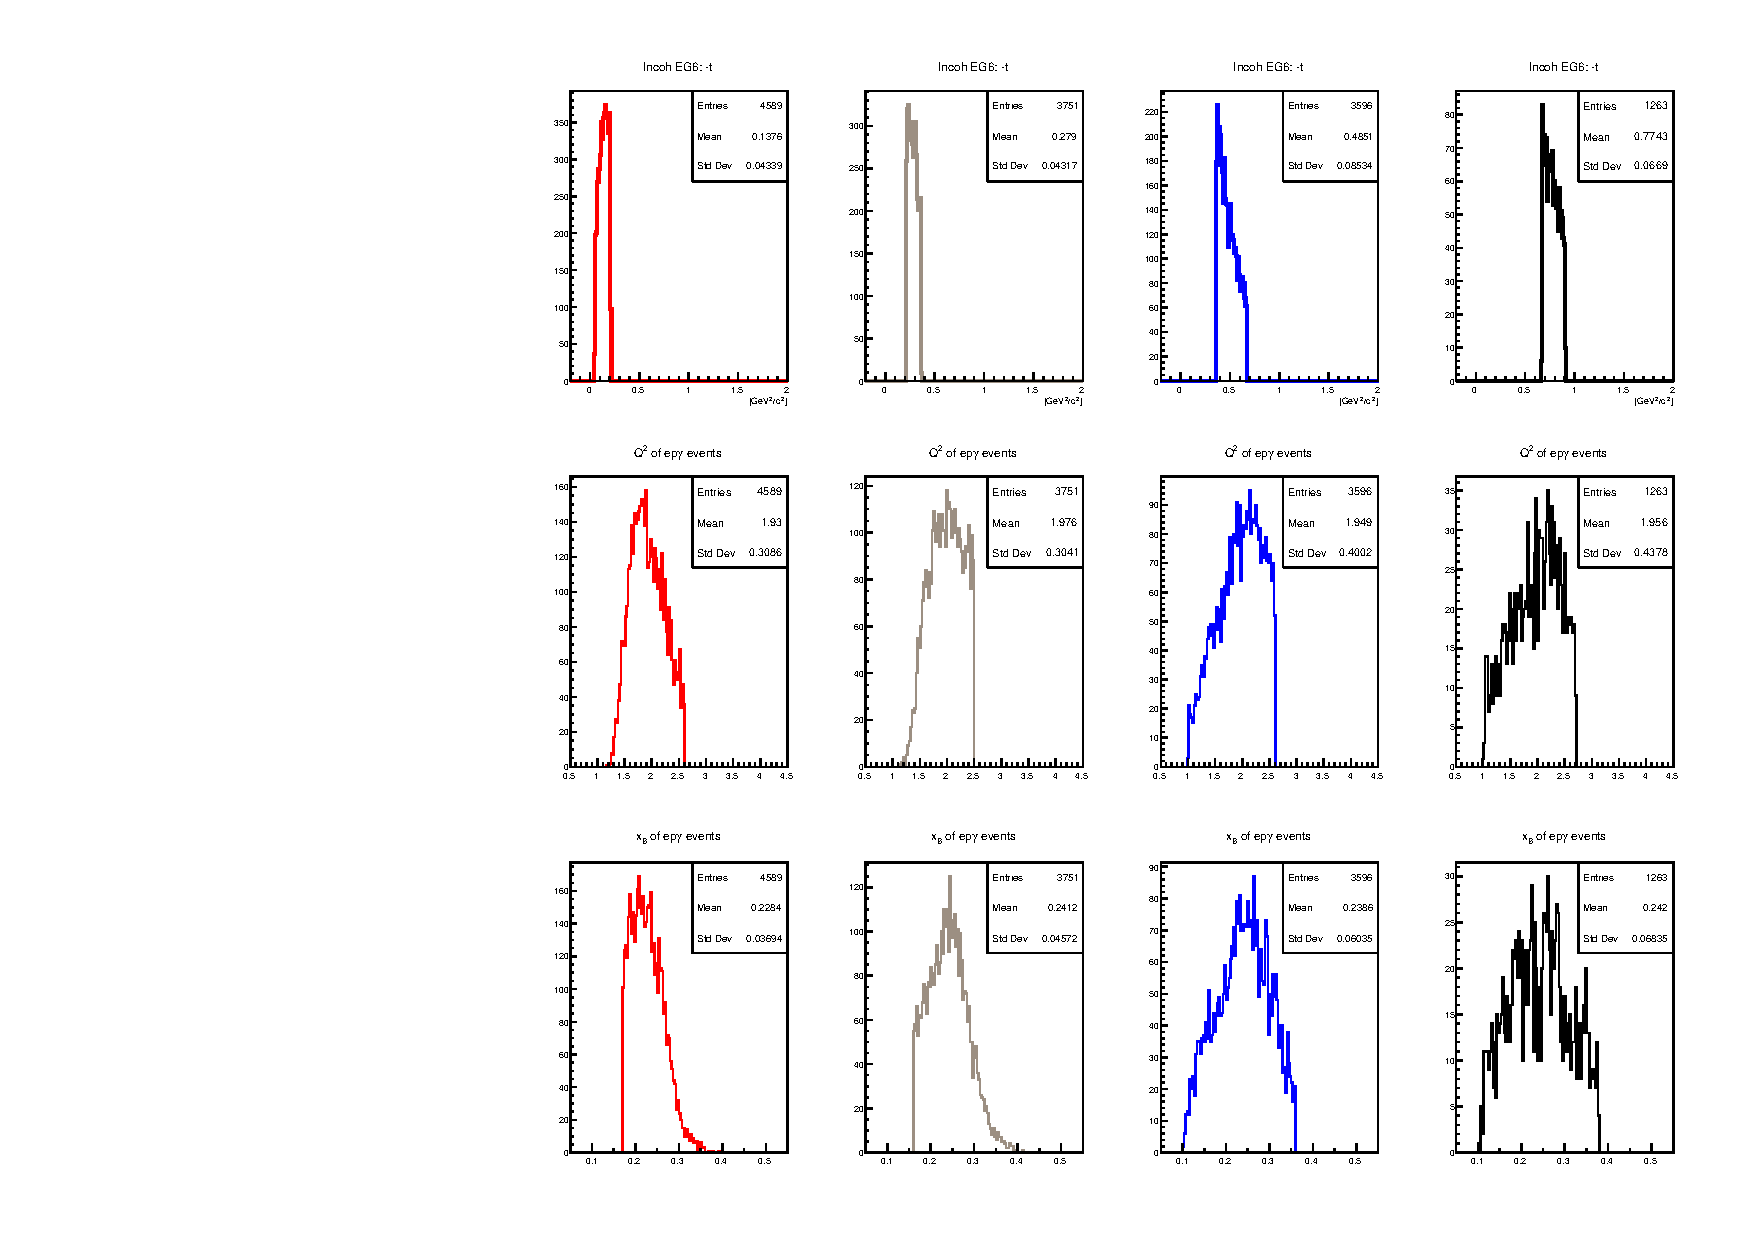
\includegraphics[width=14.9cm]{t_InCoh_bins.pdf}
   \caption{The t, $Q^2$ and $x_{B}$ distributions for the incoherent DVCS bins 
   shown in figure 6 in the prl.}
\label{fig:incoh-kin}
\end{figure}

\begin{figure}[h!]
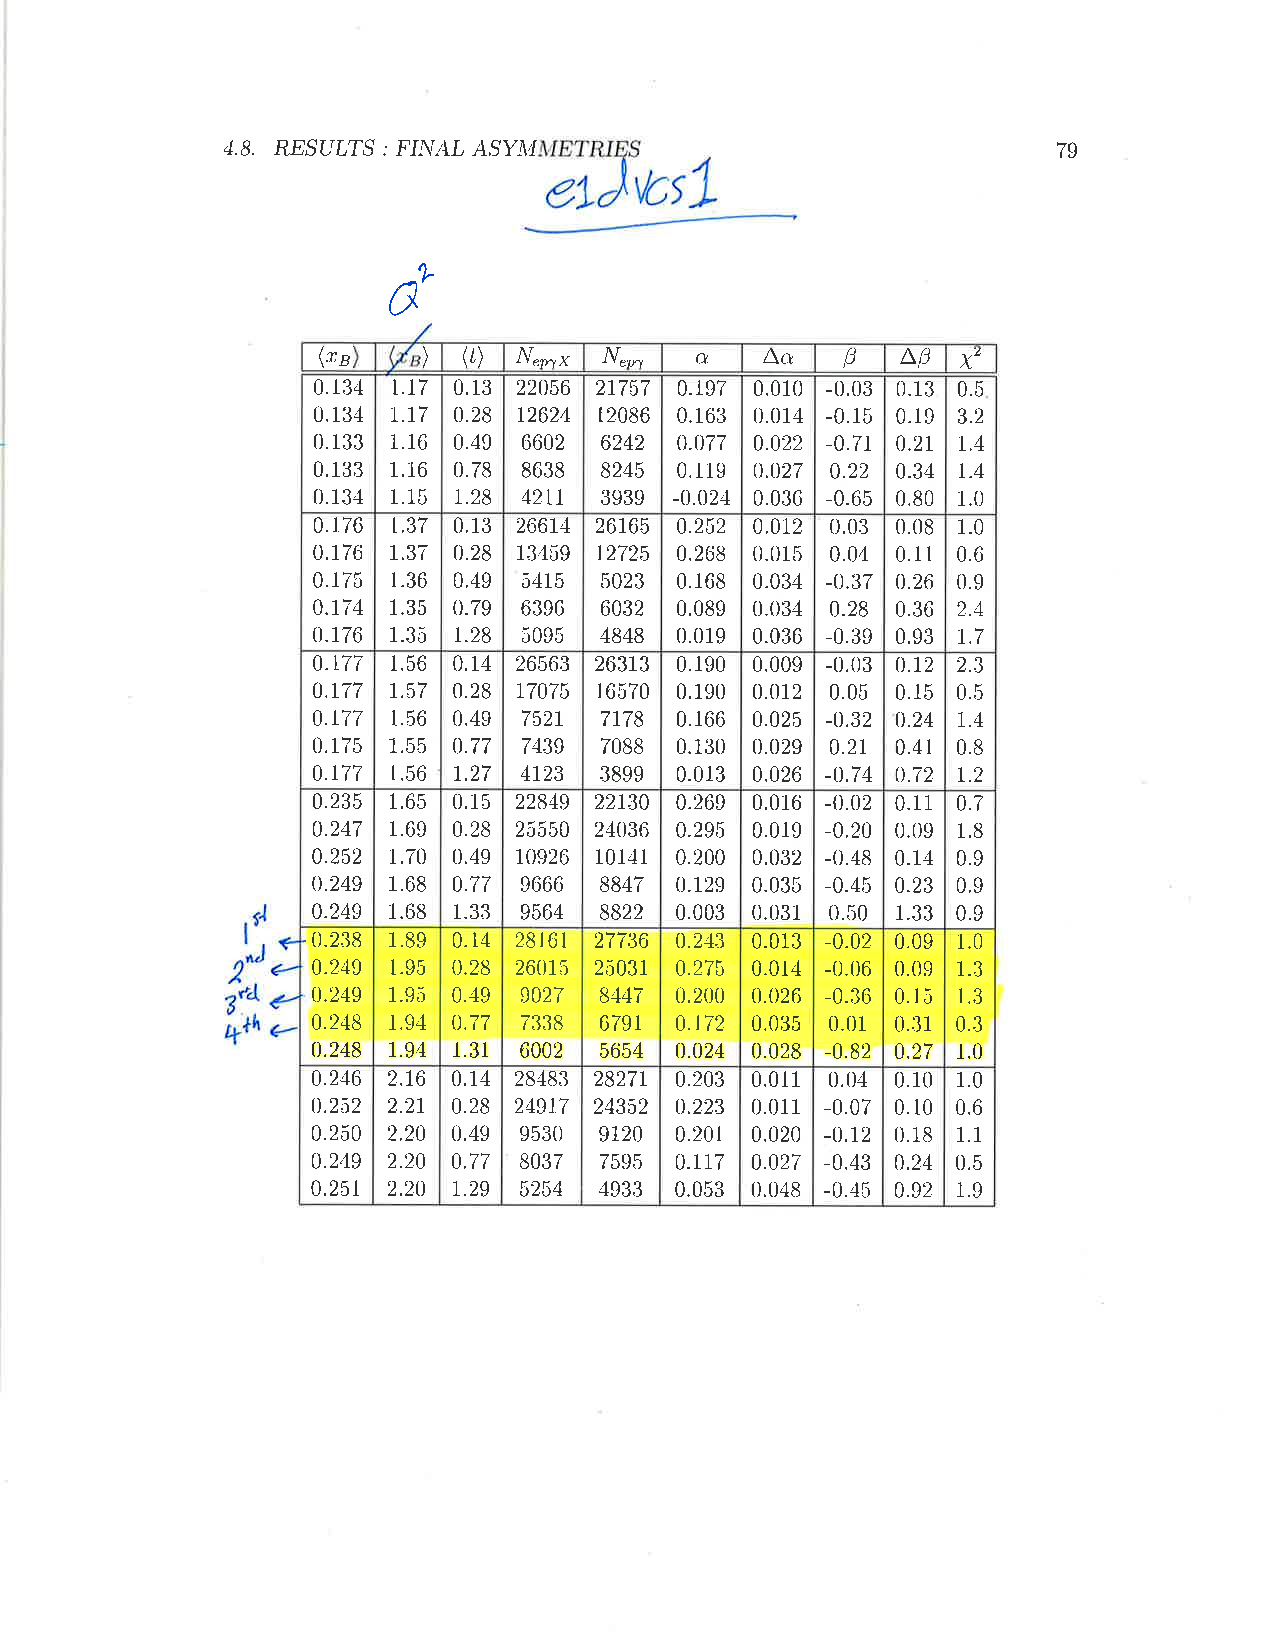
\includegraphics[width=14.9cm]{e1dvcs1_free_proton_alu.pdf}
   \caption{The free proton published beam-spin asymmetries. The highlighted 
   data points are the ones used to construct the beam-spin asymmetry rations 
   in FIG.~6 in the PRL.}
\label{fig:free-p}
\end{figure}



\item  The paper makes no mention of the initial momentum of the struck 
   nucleon, which I would expect to smear out the kinematics. It would be 
      useful for the reader to get an impression on how large this effect would 
      be. Does this explain the widths of the distributions in figure 2, or are 
      these widths dominated by detector resolution?\\
   \textcolor{blue}{We have studied this effect in details. The review 
      committee members are invited to check appendix H in the analysis note 
      \url{ 
      https://www.jlab.org/Hall-B/shifts/index.php?display=admin&task=paper_review&rid=7619165&operation=view}.}

\item  There is also no mention of final state interactions in the paper. It is 
   not obvious to me that the FSA should be zero for a beam spin asymmetry on 
      4He. If you have a calculation that shows this is the case, it would be 
      good to mention it.\\
   \textcolor{blue}{There are no such theoretical calculations of the FSI on 
      the incoherent DVCS asymmetries on the $^4$He. }

\end{enumerate}


\newpage
\newpage
\newpage
\newpage

There are also number of minor initial edits and stylistic suggestions that we 
would like you to consider. This list is in chronological order:

\begin{enumerate}
  
\item    In the title, add an "a":  "Deeply Virtual Compton Scattering off a bound proton", or make proton plural (protons).\\
   \textcolor{blue}{Updated. "protons"}

\item    First sentence of abstract, does "measurement of incoherent deeply 
   virtual..." work better?\\
   \textcolor{blue}{Updated. }

\item    Third sentence, replace "have been compared" with the more active "are compared"\\
   \textcolor{blue}{Replaced. }

\item    Line27: leave out "the fact"\\
   \textcolor{blue}{Cleaned. }

\item    Rephrase line 34. Perhaps:  "correlations can be revealed"\\
   \textcolor{blue}{Cleaned. }

\item    Line 46 - 49: Perhaps make it more clear that in the coherent case the scattering is off the entire nucleus, and that for the incoherent case the nucleon is ejected? Is that a correct interpretation of what is going on?\\
   \textcolor{blue}{Updated.}

\item    Line 78: "amplitude that contains", or make amplitude plural.\\
   \textcolor{blue}{Cleaned.}

\item    Line 154, you do not define what was used for $t_{min}$, and how it 
   was determined.\\
   \textcolor{blue}{The definitions is added.}

\item    Line 206: To make it more clear to the reader what you are doing with 
   the data, you should explicitly state that you make a fit of the $\phi$ 
      distributions, and then extract the $a_0$ value as $A_{LU}$(90). You 
      should also explicitly state that when plotting versus one kinematic 
      variable, you integrate over all the other kinematic variables. This 
      relates to comment \#2 above.\\
      \textcolor{red}{Cleaned. ( I am not sure this is needed as it is 
      mentioned at the beginning of the paragraph).}

\item    Line 207: "Fig 4 presents ..." and line 215: "We present in Fig 5". 
   One is passive, the other active. It is probably better to choose one or the 
      other, but not mix them.\\
   \textcolor{blue}{Cleaned.}

\item    Line 221: Either "Their model uses a nuclear spectral function" or 
   "Their model uses nuclear spectral functions".\\
   \textcolor{blue}{Cleaned.}

\item    Line 238: -> "on a free proton target".\\
   \textcolor{blue}{Corrected. }

\item    Line 241: "ratios show 20\%-40\% lower asymmetries" (drop "a")\\
   \textcolor{blue}{Corrected.}

\item    Line 243: rewrite to not have "effect" twice in the sentence so close together.\\
   \textcolor{blue}{Cleaned.}

\item    Line 260: Rewrite your last sentence. Suggestion: "This surprising 
   result opens a new avenue for progress in understanding quarks and gluons in 
      the nuclear medium."\\
   \textcolor{blue}{Added.}  
  
\end{enumerate}


\end{document}
